%----------------------------------------------------------------------------------------
%	PACKAGES AND DOCUMENT CONFIGURATIONS
%----------------------------------------------------------------------------------------

\documentclass[
  paper=a4,                         % Paper format
  fontsize=11pt,                    % Fontsize
  DIV=12,                           % Divided page horizontally and vertically
  BCOR=10mm,                        % Binding correction
  twoside=true,                     % Double or one-sided typesetting
  parskip=half,                     % Parskip
  headings=small,                   % small font size for headings
 ]{scrartcl}

\usepackage[utf8]{inputenc}         % Input caracters
\usepackage[T1]{fontenc}            % Font encodings
\usepackage[ngerman]{babel} 		% Language

\usepackage[document]{ragged2e}     % Textausrichtung -> Alles flushleft

\usepackage{tabularx}
\usepackage{booktabs}

\usepackage{scrlayer-scrpage}
\pagestyle{scrheadings}
\clearscrheadfoot
\pagenumbering{arabic}
\cfoot{\pagemark}

\usepackage[version=3]{mhchem} % Package for chemical equation typesetting
\usepackage{siunitx} % Provides the \SI{}{} and \si{} command for typesetting SI units
\usepackage{graphicx} % Required for the inclusion of images
\usepackage{natbib} % Required to change bibliography style to APA
\usepackage{amsmath} % Required for some math elements 

\setlength\parindent{0pt} % Removes all indentation from paragraphs

%\renewcommand{\labelenumi}{\alph{enumi}.} % Make numbering in the enumerate environment by letter rather than number (e.g. section 6)

%\usepackage{times} % Uncomment to use the Times New Roman font

%----------------------------------------------------------------------------------------
%	DOCUMENT INFORMATION
%----------------------------------------------------------------------------------------

\title{\huge Meeting Minutes \\ Zwischenpräsentation} % Title

\author{Cyrano Golliez} % Author name

\date{8 April 2020}

%----------------------------------------------------------------------------------------
%	DOCUMENT START
%----------------------------------------------------------------------------------------

\begin{document}

%----------------------------------------------------------------------------------------
%	TITELPAGE
%----------------------------------------------------------------------------------------

\maketitle % Insert the title, author and date

\vspace{1.5cm}

\begin{center}
\begin{tabular}{@{} l r @{}} \\   
\toprule
\textbf{Teilnehmer}: \hspace*{7.9cm} & Prof. Dr. Bryan T. Adey 
\vspace{1mm} \\
		   				  			 & Dr. Claudio Martani 
\vspace{1mm} \\
		   				  			 & Cyrano Golliez     
\vspace{1.5cm}  				  					       \\
\textbf{Uhrzeit}: 	                 & 10:00 - 10:30	   \\
\textbf{Ort}:		                 & Zürich				\\
	   				 
\bottomrule			   
\end{tabular} 
\end{center}

% If you wish to include an abstract, uncomment the lines below
%\begin{abstract}
%Dieser kurze Bericht umschreibt die Besprechung der Zwischenpräsentatation von Cyrano Golliezn am 8 %April 2020. 
%\end{abstract}

\vspace{1cm}

\renewcommand{\contentsname}{Übersicht}
\tableofcontents

%----------------------------------------------------------------------------------------
%	END TITELPAGE
%----------------------------------------------------------------------------------------

\newpage

\setcounter{page}{1}

%----------------------------------------------------------------------------------------
%	SECTION 1
%----------------------------------------------------------------------------------------

\section{\large Problemlösungszyklus}

Der Problemlösungszyklus soll verstärkt in die Arbeit mit einfliessen. \\ Die einzelnen \mbox Schritte sollen einen Rahmen für die Struktur der Arbeit schaffen. Mithilfe dieser strukturierten Projektbeschreibung sollte es ermöglicht werden, die Argumentation für die einzelnen Varianten qualitativ hochwertig darzulegen.  

%----------------------------------------------------------------------------------------
%	SECTION 2
%----------------------------------------------------------------------------------------

\section{\large Zielfunktion}

\begin{description}
\item[Konkrete Ziele] \hfill \\
\vspace{2mm}
Die Ziele, die ich mit dieser Intervention erreichen möchte, müssen klar ersichtlich ausformuliert werden, um eine Rahmenbedingung für die Bewertung der Varianten zu schaffen. Dies sollte helfen, die im letzten Schritt der Arbeit generierten Quantitativen Annahmen zu den entstandenen Kosten der einzelnen Varianten, mit den Anforderungen an die Infrastrukturintervention zu vergleichen. Somit können qualitative Argumente zur Bewertung der einzelnen Varianten erarbeitet werden. Diese sollen sich auf die von mir, im Rahmen der Analyse der STEK, erarbeiteten Ziele zur Verbesserung der Verkehrssituation in Uster, abstützen könne.

\begin{itemize}
\item Anreize schaffen auf das Velo umzusteigen $\rightarrow$ Nachfragesteigerung
\item Nutzung des MIV soll weniger schmackhaft machen $\rightarrow$ Nachfragereduktion
\item Der zukünftigen gesteigerten Nachfrage gerecht werden $\rightarrow$ Angebotssteigerung
\end{itemize}

\item[Allgemeine Situation] \hfill \\
\vspace{2mm}
Die von mir definierte Zielfunktion soll, mit der der allgemeinen Situation in Uster verknüpft werden. Mit der allgemeinen Situation ist hier die Wahrnehmung der Verkehrslage und die Stimmung der Bevölkerung sowie der Pendler, gemäss der Angaben der STEK im Jahr 2020, gemeint.  \\
Dies bedeutet, dass dargelegt wird, wie die allgemeine Situation im Bereich dieser Infrastruktur dazu geführt hat, dass ich mich dazu entschieden habe, für diese Infrastruktur eine Intervention auszuarbeiten. Dies sollte mit helfen eine qualitativ hochwertige und breit abgestützte Argumentation für meine Intervention zu erarbeiten..

\item[Wahl der Zielfunktion] \hfill \\
\vspace{2mm}
Die Wahl der Zielfunktion und der Komponenten der Kostenberechnung sollte klar dargelegt werden. Diese Wahl sollte mit stichhaltigen Argumenten begründet werden.
Die Zielfunktion soll so aufgebaut und begründet sein, dass sie für alle beteiligten Parteien repräsentativ ist. Sie sollte alle relevanten Kosten der wichtigsten Steakholder beinhalten und die getroffene Einschränkung auf die gewählten Steakholder und Kosten muss begründet werden.\\
\end{description}

%----------------------------------------------------------------------------------------
%	SECTION 3
%----------------------------------------------------------------------------------------

\section{ \large Richtlinien}
Mithilfe der Richtlinien der STEK soll definiert werden, welche Auswirkungen die Intervention auf die Infrastruktur haben soll. Dies sollte mit den Leitzielen der Stadtentwicklung 2035 verknüpft werden, um dadurch die Argumentation zu bekräftigen, wieso ich mich im Rahmen der Zielsetzung ''die allgemeine Verkehrssituation in Uster nachhaltig zu verbessern'', für diese Intervention entschieden habe. Es sollte somit einem objektiven Betrachter, in diesem Falle z.B. einem Mitglied des Ustermer Stadtrates ersichtlich werden, wieso ich mich für diese Infrastrukturintervention entschieden habe.
Um diese Argumentation zu bekräftigen soll dargelegt werden, was in Zukunft in Uster gemäss der STEK effektiv angepasst wird und was für Effekte diese Veränderungen auf die wichtigsten Parameter meiner Infrastruktur haben. \\
Dies bedeutet zum Beispiel, welchen Einfluss die geplanten oder sich schon im Bau befindlichen Infrastrukturveränderungen auf die Veloverkehrsmenge, die Unfallhäufigkeit sowie die Reisezeit auf den von mir untersuchten Infrastrukturabschnitt haben.


%----------------------------------------------------------------------------------------
%	SECTION 4
%----------------------------------------------------------------------------------------

\section{\large Argumentation}

\begin{description}
\item[Im grösseren Kontext] \hfill \\
\vspace{2mm}
Da in einer Diskussion über das Projekt auf gefundene Kritikpunkte eingegangen werden muss, sollte die geführte Argumentation breit abgestützt sein. Dies bedeuted, dass so viele Punkte wie möglich, in der Begründung der Wahl der Zielfunktion sowie in der Beurteilung der Situation berücksichtigt werden sollten. 

\item[Qualitativ aufwerten] \hfill \\
\vspace{2mm}
Die Argumentation qualitativ aufzuwerten bedeutet, dass für den Aufbau der Argumentation möglichst viele und insbesondere die wichtigsten Informationen miteinbezogen werden und dass sie eine breite Informationsbasis erhält. Dadurch wird es im Rahmen einer Diskussion möglich sein, die geforderten Informationen wiederzugegeben und allfällige voreingenommene Parteien vom Nutzen meiner Intervention zu überzeugen. \\ 

\item[Was sollte gemacht werden] \hfill \\
\vspace{2mm}
Es sollte dargelegt werden, was ich bei jeder Variante an der Infrastruktur zu verändern plane. Die Varianten sollten, in Anbetracht der aktuellen Strassenlage, hinsichtlich ihrer Machbarkeit diskutiert werden und sie sollten dementsprechend ausgearbeitet werden. Dies bedeuted, dass qualitativ gezeigt werden sollte, was die Durchführung der Variante für Effekte auf die ''urbane Strassenraumgestaltung'', gemäss der Richtlinien der STEK, haben könnte. Diese Richtlinien fordern, dass es genügend Platz für Fussgänger, Fahrradfahrer, den MIV sowie den ÖV als auch für Bäume und sonstige Grünanlagen am Strassenrand hat. Die Varianten müssen so ausgearbeitet sein, dass sie diese Forderungen erfüllen können. Im Falle einer alternativen Strassenraumgestaltung sollte erklärt werden, wieso diese Leitziele nicht oder anders erreicht werden. 
\end{description}
%----------------------------------------------------------------------------------------
%	SECTION 5
%----------------------------------------------------------------------------------------

\section{\large Wichtige Anmerkungen}

\begin{itemize}
\item Verallgemeinerungen für die Kostenberechnung erwähnen
\begin{itemize}
\item Referenzquellen angeben $\rightarrow$ Viele Annahmen treffen
\end{itemize}
\end{itemize}

\begin{itemize}
\item Der aktuelle Stand der Arbeit entspricht dem einer Vorstudien Phase \\
\begin{itemize}
\item Im Task 5 der Arbeit soll erwähnt werden, was ich noch hätten machen könne, um die Arbeit wie eine Detailstudie zu gestalten
\end{itemize}
\end{itemize}

\begin{itemize}
\item Was waren die Annahmen und Probleme \\ 
\begin{itemize}
\item Was wäre noch zu analysieren, wenn ich noch weiter in die Tiefe gegangen wäre.
\end{itemize}
\end{itemize}


\begin{itemize}
\item Mithilfe dieser kritischen Analyse und Reflexion soll ich meine Argumentation für die Intervention verbessern und allenfalls erweitern
\begin{itemize}
\item So dass, in einer allfälligen Diskussion, keine Punkte angesprochen werden können, die ich nicht in meiner Argumentation bereits erwähnt habe
\end{itemize}
\end{itemize}

\begin{itemize}
\item Auf die Genauigkeit achten
\end{itemize}


\newpage

%----------------------------------------------------------------------------------------
%	SECTION 6
%----------------------------------------------------------------------------------------
%\begin{figure}[!hbpt]
%\centering
%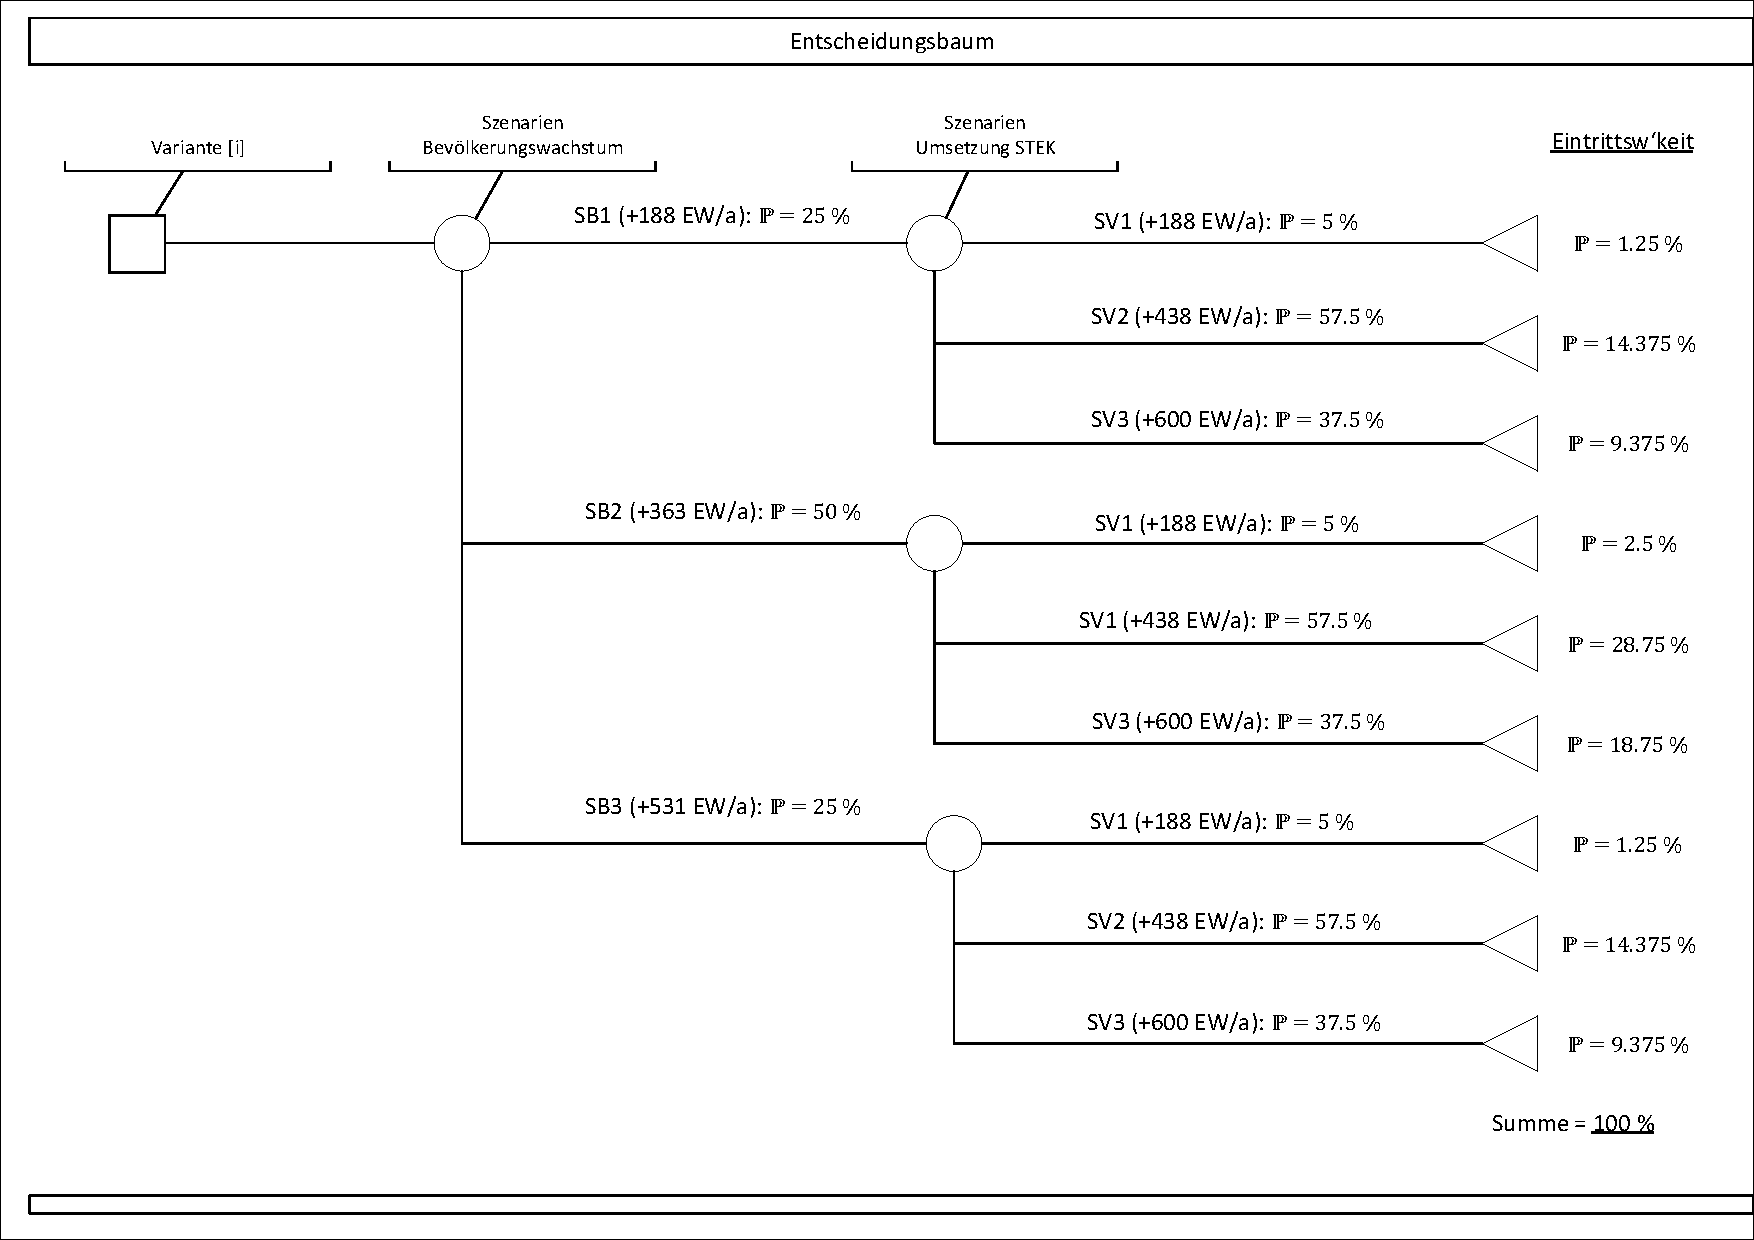
\includegraphics[width=14cm]{figures/Entscheidungsbaum(PDF)}
%\caption{Entscheidungsbaum}
%\end{figure}
%----------------------------------------------------------------------------------------
%	BIBLIOGRAPHY
%----------------------------------------------------------------------------------------

%\bibliographystyle{apalike}

%\bibliography{sample}

%----------------------------------------------------------------------------------------



\end{document}